\documentclass{ou-report}
%% \citestyle{agu}

\newcommand{\HJ}[1]{{\color{red} HJ: #1}}
\newcommand{\todo}[1]{{\color{red} TODO: #1}}
\newcommand{\vraag}[1]{{\color{teal} {\textbf{VRAGEN AAN HUGO: }}#1}}
\newcommand{\outline}[1]{{\color{blue} #1}}
\newcommand{\old}[1]{{\color{gray} #1}}

\usepackage{float}
\usepackage{tikz}
\usetikzlibrary{positioning}
\usepackage{graphicx}

% Dit template is gemaakt door P.J. Molijn in het kader van zijn afstuderen aan de OU in 2014.
% Waarvoor hartelijk dank.
% Minieme maar belangrijke wijzigingen zijn aangebracht door E.M. van Doorn
% Het template is versimpeld door Sylvia Stuurman, 2019.


%\hypersetup{
%pdfsubject={Master Thesis <Titel>, <author>},
%pdfkeywords={keyword1, keyword2}
%}

\begin{document}
\pagestyle{plain}
\title{Applying outlier detection on the scientific publication process to support fraud detection}
\author{Ewoud Westerbaan}
%Title of the thesis
%\title[Subtitle]{Title}
%\author{author}
%\affiliation{
%\begin{tabular}{ll}
%Student: & studentnumber \\
%Date:    & DD/MM/YYY \\
%\end{tabular}
%}
%
%%\coverimage{cover/cover.jpg}
%%            ===============
%\makecover[frontboxwidth=4.6in]
\begin{titlepage}

\begin{center}

%% Insert the OU logo at the bottom of the page.
\begin{tikzpicture}[remember picture,overlay]
    \node at (current page.south)[anchor=south,inner sep=0pt]{
        
\includegraphics[scale=0.7]{cover/logo}
    };
\end{tikzpicture}

%% Extra whitespace at the top.
\vspace*{2\bigskipamount}

%% Print the title in specific color.
{\makeatletter
%\titlestyle\color{ou-cyan}\Huge\@title
\titlestyle\color{red}\Huge\@title\par
\makeatother}

%% Print the optional subtitle in black.
{\makeatletter
\ifx\@subtitle\undefined\else
    \bigskip
    \titlefont\titleshape\LARGE\@subtitle
\fi
\makeatother}

\bigskip
\bigskip

by
%door

\bigskip
\bigskip

%% Print the name of the author.
{\makeatletter
\titlefont\Large\bfseries\@author
\makeatother}

\vfill

in partial fulfillment of the requirements for the degree of
%in overeenstemming met de vereisten voor het verkrijgen van de graad van

\bigskip
\bigskip

{\bfseries Master of Science}

in Software Engineering

\bigskip
\bigskip

at the Open University, faculty of Management, Science and Technology \\
Master Software Engineering
%aan de Open Universiteit Nederland,

to be defended publicly on Day Month DD, YYYY at HH:00 PM.
%in het openbaar te verdedigen op dinsdag 9 september om 15:00 uur.

\vfill

\begin{tabular}{lll}
%% Add additional information here, per faculty requirements, e.g
    Student number: & 852069942 \\
    Course code: & IMA0002\\
    Thesis committee:
        & titles and name of the chairman (chairman), & Open University \\
        & titles and name of the supervisor (supervisor), & Open University
\end{tabular}

%% Only include the following lines if confidentiality is applicable.
\bigskip


\bigskip

\end{center}

\end{titlepage} 


%% Use Roman numerals for the page numbers of the title pages and table of
%% contents.
\pagenumbering{roman}
%% Include an optional title page.

\frontmatter 


\let\cleardoublepage\clearpage

% Optional Dedication, Acknowledgement
%\input{dedication}

%\input{acknowledgement}
\tableofcontents

%Optional: list of figures, list of tables
%\listoffigures

%\listoftables

%% Include an optional summary page.
%\input{Summary/summary}
%\input{Summary/samenvatting}

\mainmatter
\pagenumbering{arabic}


\newcommand{\mi}[1]{\ensuremath{\mathit{#1}}}
\newcommand{\authors}{\mi{authors}}
\newcommand{\cites}{\mi{cites}}
\newcommand{\receives}{\mi{receives}}
\newcommand{\reviews}{\mi{reviews}}
\newcommand{\accepts}{\mi{accepts}}
\newcommand{\rejects}{\mi{rejects}}
\newcommand{\editorinchief}{\mi{EiC}}
\newcommand{\associateeditor}{\mi{AE}}
\newcommand{\Humans}{\mi{Humans}}
\newcommand{\Reviewers}{\mi{Reviewers}}
\newcommand{\Editors}{\mi{Editors}}


% ==============================================================================
\chapter*{Abstract}
% ==============================================================================
% Placeholder

\outline{
\begin{itemize}
    \item Geen nummering
    \item voor introductie
    \item Probleem
    \item Main contributions
    \item Main results
\end{itemize}
}

% ==============================================================================
\chapter{Introduction}
% ==============================================================================
\outline{
\begin{itemize}
    \item Wat moet een informaticus met een andere focus weten om deze scriptie 
        te kunnen lezen.
\end{itemize}
}
\outline{
    er bestaat fraude, sommige worden gevonden, blabla (smeuig maken)
}
Incentives for scientists rely on quantitative measures of science, such as 
number of publications, number of citations and amount of grants received. 
However, as the aphorism known as Goodhart's Law states: ``When a measure 
becomes a target, it ceases to be a good measure''~\cite{strathern_1997}. That 
is the case here as well: these metrics not only incentivise scientific 
excellence by doing research and publishing the results; they also invite 
, maybe even more rewarding, dishonest approaches to achieve high rankings 
-- gaming of these metrics, or, more simply, fraud in scientific publishing. 
Examples of such fraud include plagiarism, manipulation of images (e.g., of cell 
extracts in life science publications), manipulation of research data, 
fabrication of research data. In addition, there may be as-of-yet unknown forms 
of fraud.

Various prevention and detection measures are in place. In absence of these 
deterrents, the scientific process would be vulnerable to dishonest behaviour. 
These existing deterrents are typically focused on specific forms of dishonest 
behaviour. Examples of these existing measures are Ithenticate to detect 
plagiarism, or ORI's Forensic Droplets\footnote{\url{https://ori.hhs.gov/droplets}} 
to detect manipulated images. The practice of preregistration ensures scientific 
studies are conducted as planned, and help to prevent data manipulation such as 
p-hacking\footnote{P-hacking is manipulation of the data so the research becomes 
statistically important.}. Another measure is applying statistical evaluation to 
uncover manipulation of research data~\cite{HGWA2019}. 

Despite these deterrents, some forms of dishonest behaviour still slip through.
\HJ{eventueel hier enkele aanvallen noemen.}
Such behaviours use dishonest tricks outside the detective capabilities of
current detection methods and therefore escape initial scrutiny. We know of
such cases typically through whistle blowers and manual investigation. 
This has illustrated that there still exists a problem, yet the scale of the
problem remains unknown.
In particular, one obstacle is the huge (and growing) number of scientific 
publications and scientific authors. For example, the DBLP website, which 
records most publications in computer science, currently lists more than 
2.5~million authors -- a number that cannot be manually investigated. Hence, a 
more generic approach to detect fraud is needed. 

\todo{
\begin{itemize}
    \item dus: Generieke vorm van detectie gewenst
    \item dat kan dus niet afhangen van een specifieke aanval
    \item dat moet dus gebaseerd zijn op een holistische view van het 
        publicatieproces (kerngetallen bijvoorbeeld)
        -- en weten wat daar de norm is.
    \item Dus beschouwen we in de volgende secties het publicatieprocess in meer 
        detail.
\end{itemize}
}

In this project, we aim to take the first step in this direction by not focusing 
on the method of fraud applied, but on the \emph{effect of scientific fraud}, by
taking a holistic view of the publication process. We tend to do this in two 
steps:
\begin{enumerate}
    \item The first step is to identify groups of people sharing a 
        charateristic (e.g. same role, same H-index).
    \item The second step is to identiy outliers within this group based on
        other characteristics (e.g. number of publications).
    
    
    % The 
    % underlying assumption is that the various types of scientific fraud all 
    % share a common characteristic: their goal is the same, that is, their goal 
    % is to improve a researcher's or publication's quantitative measures of 
    % science. This elevates them above their peers -- which on the one hand 
    % brings recognition and accolades, but on the other, makes them stand out. In 
    % short, the underlying assumption is that fraudsters aim to become outliers 
    % (in terms of quantitative measures of science).

\end{enumerate}

To clarify this with an example: An editor of a journal publishes in this 
same journal. This is not a strange fact on itself. However, if other editors of
this same journal do not publish (or publish much less), we can consider this 
editor an outlier. Other examples are given in Section~\ref{interesting_cases}.

People with malicious ways to accomplish improvement of their quantitative 
measures, will be an outlier compared with their peers.

We immediately caution that this implication does not hold in reverse. That is: 
such outliers need not be fraudsters. 
However: identifying outliers may reduce the pool of authors to be investigated
by several orders of magnitude. Thus, while not perfect, outlier classification
should make manual investigation of cases where fraud would have had significant
effect possible.

The goal of this project is to take a first step to make this a possibility.
Concretely, we will design a generic detection method which uses the metrics
of the publication process and the incentives of the authors. Our proposal is to 
use machine learning techniques to detect authors which are outliers, given the 
metrics of the publication process. The goal we aim to achieve with our proposal 
is to focus the limited capacity of manual fraud investigation to strongly 
increase the probability of identifying the most egregious of fraudsters. 
% ------------------------------------------------------------------------------
The detection method which we will design is for the computer science 
discipline. For other disciplines this method probably needs to be tuned. For 
example: the average number of co-authors per article change between research 
areas\footnote{\url{https://www.natureindex.com/news-blog/paper-authorship-goes-hyper}}.

\outline{
\paragraph{Tweetrapsraketten}
% -------------------------------------
Idee: (1) vind groep personen; (2) vind outliers binnen die groep
\begin{itemize}
\item Editors van hetzelfde journal $\implies$ \#pubs in journal
\item Mensen met zelfde H-index  $\implies$
    \begin{itemize}
    \item \#publicaties
    \item \#jaren actief
    \item \#citaties in h-core (hoeveel papers hebben minimale score) \\
        Dit is een beetje: hoe verloopt de citatie``curve'' vergeleken met anderen
    \item ranking van venues in h-core
        \begin{itemize}
        \item In vergelijking met anderen
        \item In vergelijking met papers buiten je eigen h-core \\
            en dan ook in vergelijking met anderen
        \end{itemize}
        
    \end{itemize}
\end{itemize}
}
\section{Contributions}
\outline{
\begin{itemize}
    \item Wat gaan wij bijdragen en waarom is dit cool? -> Motivatie
    \item +/- 1 contributie per hoofdstuk
\end{itemize}
}
During this research we will contribute the following items to the community.
\begin{description}
    \item[Situations of dishonest behaviour] which we want to identify using our 
        methodology; the attacks.
    \item[A formal model of the publication process] which contains the objects 
        necessary to catch the identified attacks.
    \item[Data collection methodology] to get the necessary data to provide an 
        holistic view on the publication process.
\end{description}
\old{
\begin{description}
    \item[A formal model of the publication process] The publication process 
        consists of inputs (features) and outputs (metrics). Simply defined; the 
        output is depended on the inputs, and those inputs are a result of the 
        behaviour of the author. The output is the metric the author want to 
        change in his (or her) favor. To determine what features we need to 
        monitor, we need to understand how this publication process works. To 
        achieve this, we need to have a formal model of the process to analyse 
        these relations, which is our second contribution:
    \item[Deriving input-output relations] Given this formal model, we can 
        derive all inputs that affect the output metrics, which are the metrics 
        an attacker wants to adjust. This is important because these relations 
        give us insights how the publication model can be played. With the 
        inputs of these relations we can start putting together a list of 
        features we need to collect. We will formalise a few metrics and 
        elaborate how to game this model to adjust them in favor of the 
        attacker. Except these theoretical gaming, we also know some attacks on 
        the model which actually did took place, which leads to our third 
        contribution.
    \item[Overview of known attacks] We investigate known attacks and show how 
        to model these attacks in the formal model. This substantiates that the 
        formal model is relevant for detecting practical attacks. Combining 
        these with the formal attacks brings us to our fourth contribution.
    \item[Features indicating an attack] We combine the knowledge gained from 
        establishing input-output relations and the theoretical embedding of 
        practical attacks in the formal model to derive features that are 
        indicative of metrics, and therefore, possibly abused in attacks. Having 
        this features, we can proceed with the detection method.
    \item[Detection method] With these features in hand we propose a formal 
        approach to automatically separate ``interesting'' cases from regular 
        scientists. Consider these features as input for our detection 
        mechanism, the output is a set of regular authors and a set of authors 
        that are positive outliers on (combinations of) those features.
\end{description}
}


    
% This research proposal continues in Section~\ref{RelatedWork}, 
% \nameref{RelatedWork}, where we discuss publications which are related to the 
% goal we want to achieve. A major topic in this project is outlier (or anomaly)
% detection; we will discuss this topic and how this incorporates in this project 
% in Section~\ref{anomaly_detection}. Next, we describe our research questions in
% Section~\ref{Research_ResearchQuestions} and how we think we should be able to 
% answer them in Section~\ref{Research_ResearchMethod}. Because the research we 
% propose is very dependent on data, we provide an initial investigation of 
% possible data sources. The outcome and result of this analysis is described in 
% Section~\ref{Research_Data} '\nameref{Research_Data}'. The validity of our 
% research is discussed in Section~\ref{Research_Validation}. The research
% proposal concludes with a planning in Section~\ref{Planning} and risks and 
% mitigation strategies in Section~\ref{Planning_RiskAnalysis}.






% ==============================================================================
\chapter{Domain analysis of the publication process}
% ==============================================================================
\outline{
\begin{itemize}
    \item Beginnen met verhaal over publicatieprocess
    \item Reden: wetenschapper wilt publiceren
\end{itemize}
}

Incentives for scientists rely on quantitative measures of science, such as 
number of publications, number of citations and amount of grants received. This 
gives scientist a higher status, salary, more resources (funds, students) to do 
more research (which leads to more rewards); recognition and accolades. To 
achieve these rewards, scientists need to have their papers published for their 
career to thrive. This process of publishing and rewarding is shown by Bj\"ork 
and Hedlund~\cite{BH2004} in a cycle within their visualisation of the 
publication process. In Figure~\ref{fig:publish_incentives} we present this 
cycle.

\begin{figure}[H]
\centering
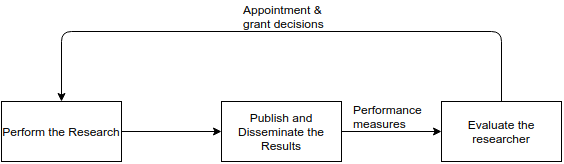
\includegraphics[width=12cm]{images/publication_process.drawio.png}
\caption{Publish for incentives (adapted from~\cite{BH2004})}
\label{fig:publish_incentives}
\end{figure}
% ==============================================================================

In this image we see that the researcher is evaluated and receives incentives 
(such as funds) based on performance measures. In their paper,  Bj\"ork and 
Hedlund mention that for public bodies that provide funds (which is an incentive 
for the researcher), the production and consumption of publications should be 
optimized.
% For researchers, there are multiple strategies to achieve appointments and grants.
% Interestingly, only one of these is to act honestly, that is, to perform the
%     research and publish results. Dishonest approaches are possible,
%     and may even be more rewarding. In absence of deterrents, the scientific
%     process would be inundated by this.
%     \todo{naar intro}
% Existing deterrents are typically focused on specific forms of dishonest
%     behaviour. However, dishonest behaviour still occurs.
    


%% For an author this is an interesting perspective. What can we consider 
%%     production and what consumption and, for detecting fraud, how can we pretend 
%%     to produce and pretend the work is being consumed. In other words; how can 
%%     one pretend to be interesting and gain incentives.
%%     % \item It is save to consider bringing papers to the public as publication. In this chapter we will dive in how this process looks like and the roles and power involved; who has the power that your work can even be consumed?
Two main targets exists for scientific publication: journals (incollection) or 
conferences (inproceeding). While journal publications are the norm in many 
other disciplines, conference publications are common in Computer Science.

The next sections describe these processes from a Computer Science perspective. 
For other disciplines these processes may differ. For example, in CS 
conferences, rigorous peer-review is the norm, with acceptance rates of 20\% or 
less being common; in other disciplines, peer review may be less strict.
    
In the next section we examine the process in more detail.


% ==============================================================================
\section{Journal publication}
\outline{
beschrijvend het process bespreken
}

First we will discuss the process for publishing in a journal. Although the 
exact process may differ across journals, there is a certain common process. We 
tend to describe this common process.

The process of publishing in a journal starts at the author who has a manuscript 
he wants to have published. This can be based on a 'call for papers', or on own 
initiative. According to Cormode, the Editor-in-Chief receives the manuscript 
and do a minor check if the paper is good enough for further processing. If it 
is, the further process of handling the paper is assigned to an associate editor 
who also perform some checks for quality (understandability, duplication of 
prior work, topic in scope). The checks from the editor-in-chief and associate 
editor can lead to a rejection of the manuscript. According to Cormode, the 
author is encouraged to suggest an associate editor at submitting. This helps 
the editor-in-chief to delegate the handling to a associate-editor with 
knowledge of the domain e.g..

The main responsibilities of the associate editor are 1) Initial handling and 
selecting reviews for the papers and 2) obtaining a decision for a paper. 
Although selecting reviewers to review a manuscript is a responsibility of the 
associate editor, it is not uncommon for an author to suggest reviewers. 
Sometimes he even needs to provide reviewers.

After getting the results from the reviewers, the associate editor decides if 
the manuscript needs to be adjusted. Formally the reviewers give an advise, but 
it is up to the associate editor to do the final judgement. If adjustments are 
needed, the author adjusts his manuscript and this needs to be reviewed again. 
This can happen with other reviewers. An alternative path is that an author 
chooses to withdraw his paper.

Eventually, hopefully, if the paper is accepted by the associate editor, an 
advise will be given to the editor-in-chief. Formally the editor-in-chief 
decides if a paper is being published, but most of the time the advise of the 
associate editor is adopted. This chain of advise and assignment is shown in 
Figure~\ref{fig:c2013}. Interesting in this schematic overview is the absolute 
power of the Editor-in-Chief. He can make a judgement without the advise of the 
associate-editor (and reviewers). Also this role can influence the process by 
choosing a specific associate-editor. Under the Editor-in-Chief, we draw the 
Associate editor. This role has two ways to influence the process; by choosing 
the reviewers and by giving the advise to the editor-in-chief. The reviewers 
have less power; off course they can provide an advise, but most of the cases 
there are multiple reviewers.

\begin{figure}[H]
\centering
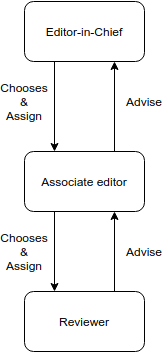
\includegraphics[width=3cm]{images/c2013.drawio.png}
\caption{Roles within the journal process (visual interpretation of description in~\cite{C2013})}
\label{fig:c2013}
\end{figure}
\outline{
wordt zo en zo laten zien in in BH
}

Bj\"ork and Hedlund modelled the various processes involved in scientific
publishing to investigate the business impact of the shift towards internet
publishing models.
This model is based on publication for journals.
For our research, we took a diagram from their publication and took the activities usable for our research.
Hereby neglecting the steps "Negotiate copyright" and "Copyedit Article". The result is shown in Figure~\ref{fig:bh2004_a22331}.


\begin{figure}[H]
\centering
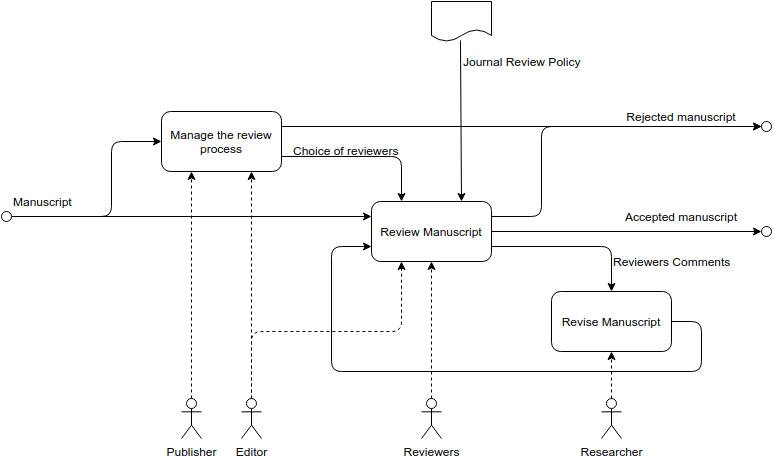
\includegraphics[width=14cm]{images/bh2004_dia_a22331_part.drawio.png}
\caption{Journal process flow between submission and decision (adapted
from~\cite[diagram A22331]{BH2004})}
\label{fig:bh2004_a22331}
\end{figure}

The phase "Manage the review process" from Bj\"ork and Hedlund is described by Cormode from the perspective of the Editor-in-Chief and Associate editor (Bjork and Hedlund decided to use one role: editor). 



\todo{blinds, double blinds om persoonlijke connecties te ondervangen}

% ==============================================================================
\section{Conference publication}
\outline{
The following is an informal description of the process for conference 
publication. This can also be a workshop or symposium. Not all conferences 
follow this approach.

For established venues the steering committee decides to have a conference and 
choose a location. The main responsibility of the steering committee is to 
oversee the organisation of the conference and choosing the program 
committee (PC) chairs which responsibility is to compose a program out of a 
subset of the received 
submissions. For new subjects, the trigger comes from one or more 
academics who thinks a conference is needed for a certain subject and try to 
form a Program Committee (PC). Possibly there are ``program tracks'' on specific 
subjects, with dedicated chairs for each track.
% ============================================================================== 
The PC chairs invite people to become program 
committee members. A new trend is self-nomination; one can nominate himself for 
a position in the program committee. Another new trend is that authors of 
submitted papers are required to review.

Besides inviting members, the PC chairs ensure the website is up, promotion 
is in place and have submission/review server set up.
The PC chairs create and distribute a call-for-papers, which starts the 
\textbf{submission phase}.
% ============================================================================== 
Responding to the call-for-papers, scientists submit papers, and possibly 
marking conflict of interest. Likely, PC Chairs extend deadline, which gives 
more scientists the possibility to submit papers. PC Chairs close submission and 
perform desk reject.
% ============================================================================== 
After the submission phase closes and the bidding phase begins. During the 
bidding phase, PC members bid on which papers they would like to review.

In the \textbf{review phase} the PC members read and score the papers. In this 
phase a paper can be early rejected with limited number of reviewers. Sometimes 
this phase contains a rebuttal phase; the reviews are send to authors so the 
authors can reply on the given comments.

In the following \textbf{discussion phase} the PC member unify their views about 
the papers.

During the \textbf{decision phase} the PC Chairs formalise a decision about a 
paper (formally; often they simply follow the consensus view). Possible 
decisions are accept, reject or conditionally accept (shepherding). In this 
case, the paper is interesting but not yet quite acceptable, salvageable. One 
reviewer is designated Shepherd and communicates with the authors on what 
changes are needed. Final acceptance hinges on the Shepherd officially 
approving the paper.

In the \textbf{camera-ready phase} the authors make final changes, 
incorporating editorial changes, reviewer comments, etc., and submit the final 
version for publication.

In the \textbf{publication phase} the PC chairs judge on the the camera-ready 
version, and papers is published online.
% ============================================================================== 
}

\paragraph{The NIPS experiment}
For scientists getting a paper in a conference is important for their career. 
Unfortunately, the NIPS experiments makes clear that reviewing papers for a 
conference is not a deterministic
process\footnote{\url{http://blog.mrtz.org/2014/12/15/the-nips-experiment.html}}.
The result if a paper is being approved depends on the composition of the 
responsible committee. This means that the committee judging papers for 
conferences has the power to determining whose paper is being accepted and 
therefore whose career is going to thrive.


\outline{
\begin{itemize}
    \item wat is macht program committee vs program chair; 
    \item Conferentie, core ranking: https://www.core.edu.au/conference-portal
    
\end{itemize}
}

% \newpage
% \subsection{Model of proceedings}
% \begin{figure}[htbp]
%   \begin{center}
%         \begin{tikzpicture}[
%             auto,node distance=5cm,thick,
%             rolenode/.style={circle, draw=green!60, fill=green!5, very thick, minimum size=1.05cm},
%             thingnode/.style={rectangle, draw=red!60, fill=red!5, very thick, minimum size=1.05cm},
%             ]
%             % Nodes
%             \node[rolenode] (sponsoring_organization) {SO};
%             \node[rolenode] (general_chair) [below=of sponsoring_organization] {GCh};
%             \node[rolenode] (general_committee) [below=of general_chair] {GCo};
%             \node[rolenode] (program_chair) [below=of general_committee] {PCh};
%             \node[rolenode] (program_committee) [below=of program_chair] {PCo};
%             \node[rolenode] (reviewer) [right=of program_committee] {R};
%             \node[rolenode] (steering_committee) [right=of general_chair] {SC};
            
            
%             \node[thingnode] (conference) [right=of general_committee] {Conference};
%             \node[thingnode] (proceeding) [below=of conference] {Proceeding};
%             \node[thingnode] (paper) [below=of proceeding, right=of reviewer] {Paper};
%             \node[rolenode] (author) [right=of proceeding] {A};

            
%             % Lines
%             \draw[->] (sponsoring_organization) -- node [text width=2.5cm,midway,above,sloped] {appoints} (general_chair);
%             \draw[->] (general_committee) -- node [text width=2.5cm,midway,above,sloped] {organizes} (conference);
%             \draw[->] (general_chair) -- node [midway,above,sloped] {assembles} (general_committee);
%             \draw[->] (general_committee) -- node [midway,above,sloped] {contains / advises for members} (program_chair);
%             \draw[->] (program_chair) -- node [text width=2.5cm,midway,above,sloped,align=center] {assembles} (program_committee);
%             \draw[->] (program_committee) -- node [text width=2.5cm,midway,above,align=center] {assigns} (reviewer);
%             \draw[->] (conference) -- node [text width=2.5cm,midway,above,sloped] {leads to} (proceeding);
%             \draw[->] (proceeding) -- node [text width=2.5cm,midway,above,sloped] {contains} (paper);
%             \draw[->] (reviewer) -- node [text width=2.5cm,midway,above,sloped] {reviews} (paper);
%             \draw[->] (author) -- node [text width=2.5cm,midway,above,sloped] {writes} (paper);
%             \draw[->] (steering_committee) -- node [text width=2.5cm,midway,above,sloped] {plans} (conference);

%         \end{tikzpicture}
%   \end{center}
%   \caption{Publication process for collections.}
%   \label{fig:structure}
% \end{figure}

% ==============================================================================
\section{Fraud in the publication process}
\outline{
\begin{itemize}
    \item Domain
    \item Impact van process Welk effect heeft publiceren
    - \# publicaties
    - \# citaties
    - kwaliteit
    \item beter doen levert voordelen
    \item dus zijn er incentives voor valsspelen
    \item Idee\"en egregious examples -> als deze situatie voorkomt, wil ik 
    het vinden
\end{itemize}
}
% ==============================================================================
As the aphorism known as Goodhart’s Law states: “When a measure becomes a 
target, it ceases to be a good measure” [Str97]. That is the case in these 
publication processes as well: these metrics not only incentivise scientific 
excellence; they also invite other ways to achieve high rankings – gaming of 
these metrics, or, more simply, fraud in scientific publishing. 

The underlying assumption is
that the various types of scientific fraud all share a common characteristic: their goal is the
same, that is, their goal is to improve a researcher’s or publication’s quantitative measures
of science. This elevates them above their peers – which on the one hand brings recog-
nition and accolades, but on the other, it makes them stand out. In short, the underlying
assumption is that fraudsters aim to become outliers (in terms of quantitative measures of
science).


\outline{
\begin{itemize}
    \item probleem -> valsspelen
    \item - wat is dat
    \item - op oneigenlijke gronden
\end{itemize}
}
% ==============================================================================
Examples of such fraud include plagiarism, manipulation of images (e.g., of cell 
extracts in life science publications), manipulation of research data, 
fabrication of research data. In addition, there may be as-of-yet unknown forms 
of fraud.

\outline{
\begin{itemize}
    \item dan interessante gevallen
\end{itemize}
}
The next section we elaborate on some interesting cases that may contain fraud.
It is certainly not the case that all situations do actually imply fraud, but 
these are cases that need further manual investigation.


\section{Interesting cases}
\label{interesting_cases}
In this section we describe theoretical and practical (actually happened) 
attacks on the integrity of the publication process. We can use these attacks to 
complete the theoretical (or logical) publication model.

% ------------------------------------------------------------------------------
\subsection{Example: Publications cites publications in same venue}
In this part we will go through a situation to describe the process of analysing
a situation which can be an attack on the publication process. The chance this 
particular situation occurs is not very high and we will
not incorporate this in our model. The reason for this is that there is a good
enough safety net to catch this situations provided by Thomson, institute that 
calculates the Journal Impact Score. Besides, in our research we are looking for
interesting persons, and we do not consider a venue a person (although in the
end someone must be responsible).

\textit{First we describe the situation and provide a model of instances that 
are involved. This can be persons in a certain role, venues, publication etc}.

Having publications citing publications from a certain venue, increases the 
journal impact factor.

We give a model of this situation in Figure~\ref{fig:cpsv}.

\begin{figure}[H]
\centering
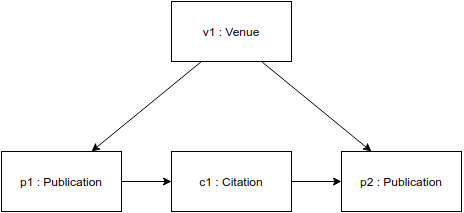
\includegraphics[width=9cm]{images/cited_publications_same_journal.drawio.png}
\caption{Instance model of citation of publication in the same venue}
\label{fig:cpsv}
\end{figure}

In Figure~\ref{fig:cpsv} we see a venue (v1) that conains a publication (p1)
which has a citation (c1) to a publication (p2) in the same venue.
% ------------------------------------------------------------------------------
\paragraph{Attack}
\textit{We describe when (this is not always the case, see 'Beneign 
alternatives') and how this situation is an attack.} 

It is not unusual that 
publications in a journal cite publications from the same venue. However, as we 
will see with most attacks, when this occurs much more 
compared with other venues and the 'self'-citation rate is higher, it becomes 
interesting. This may indicate that this is a conscientious action to increase
the Journal Impact Score, and that an attack.

\paragraph{Model impact}
\textit{In this part we describe how this situation impacts the publication 
model.}

What does in- or decrease and on what way this impacts the 'score' (or index) 
of the attacker.
The impact on the publication model is that the number of citations to 
publications in the same venue impact score of a journal raises. This number has
impact on the journal impact score.

\paragraph{Beneign alternatives}
\textit{In this part we describe how this situation can occur, while not being
an attack.} 

If a certain venue is that specialised in a certain topic, the 
situation where a publications cites other publications in that venue can occur.


% \outline{
% \begin{itemize}
%     \item The articles of a journal that are cited impact the journal impact factor.
%     \item It is important that this number is high.
%     \item Meetbaar door de verhouding te bekijken van de journals waar de geciteerde artikelen uit komen.
%     \item \todo{Wie is dan interessant? author of editor?}
%     \item In praktijk al Thomson
%     \item Verwachting is niet veel op vinden
%     \item deze laten zitten
%     \item als voorbeeld hoe de modellering werkt
% \end{itemize}
% }


% ------------------------------------------------------------------------------
\subsection{Work member of editorial board is being cited}
\label{sec:work_member_editorial_board_cited}
% The editorial board can also be the program committee in case of incollections.
When an author becomes a specialist of a certain subject, it is not uncommon 
that this person becomes member of the editorial board or program chair of a 
venue that handles this specific subject.
New publications regarding this subject will likely be published in this venue. 
It is not strange that this publication cites work of the person-of-interest, if 
he is indeed a specialist.
In Figure~\ref{fig:cweb} we present an instance model of this situation. In the 
model, pers1 presents the person-of-interest. We notice the relation of this 
person to the venue (v1) as an editor and to previous work (p2) as an author. A 
new publication (p1) has a 
citation to the previous work of the person-of-interest (c1).

\begin{figure}[H]
\centering
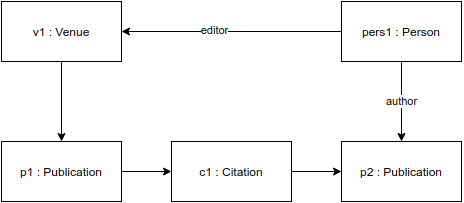
\includegraphics[width=9cm]{images/cite_work_editorial_board.drawio.png}
\caption{Instance model of citation of work of member from editorial board}
\label{fig:cweb}
\end{figure}

% ------------------------------------------------------------------------------
\paragraph{Attack} When this situation is being enforced (malicious intent), it 
becomes attack (e.g. the editor says: "cite me"). The person of interest benefits 
from being more cited. The question is now how this enforcement impacts the 
publication model so we are able to detect this. 

% ------------------------------------------------------------------------------
\paragraph{Model impact}
The impact this attack has on the publication model is on the objects Venue, 
Person (with the role editor) and the relationship between. This relationship is 
the fact that a person works for a venue. In this relationship, citations occur; 
while a person works for a venue his work is being cited. In case of an attack; 
we see more citations here than normal. The metric we need from this 
relationship is the number of citations: \textit{number\_of\_cites}. But we need 
to take the time into account; if a person works for a venue for a long time (
multiple incollection or inproceedings are published), it is logic the number of 
cites is high. Because of this; we also need the number of incollection and 
inproceedings: \textit{number\_of\_issues}.
These metrics can be used for comparison by calculating the 'normal' and the 
deviation of all editors. This normal can be calculated over the venue the 
editor is working for, or all venues. This comparison makes it possible to 
identify interesting editors.

\begin{figure}[H]
\centering
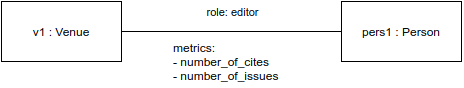
\includegraphics[width=9cm]{images/cite_work_editorial_boardmodel_impact.drawio.png}
\caption{Metrics needed for detection on publication model}
\label{fig:cwebimpact}
\end{figure}

% \begin{itemize}
%     \item Het roept vraagtekens op als gepubliceerd werk referenties bevat van iemand in de editorial board of program committee.
%     \item Dit is niet per se slecht; maar lichtelijk vreemd.
%     \item Als de persoon in de board ook in andere publicaties geciteerd wordt op het moment dat deze persoon in de board zit, wordt de twijfel of dit nog ethisch is groter.
%     \item \todo{hoog aantal gaat vraagtekens opleveren}
%     \item members onderling vergelijken
%     \item kan verschillen per venue
% \end{itemize}

% ------------------------------------------------------------------------------
\paragraph{Beneign alternatives}
The described impact on the publication model can also have other beneign reason 
to occur. The detection strategy is not foolproof. We need to take into account 
that a person is actually that good, it is logic he is being cited far more that 
its peers.

% ------------------------------------------------------------------------------
\subsection{Author reviews his own work}
This is off course a major attack on the integrity of the publication model. It 
should never be the case that an author becomes in a position where he can 
review his own work. Unfortunately, we know of such case with Moon. In 
Figure~\ref{fig:air} we present an instance model of this situation. We have one 
person (pers1) who have multiple roles in relation with one publication (p2).

\begin{figure}[H]
\centering
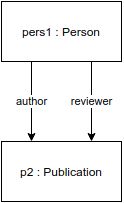
\includegraphics[width=3cm]{images/author_is_reviewer.drawio.png}
\caption{Instance model where author is also the reviewer}
\label{fig:air}
\end{figure}
% ------------------------------------------------------------------------------
From a set theory perspective we can describe this situation as: 
$\{h \in \Humans \mid \authors(p, h) \land \reviews(p, h)\}$.

In theory this situation should not be hard to found. However, besides 
availability of the necessary data, one who will execute such an attack, will 
most likely not give his own name as reviewer at submitting his paper (it is 
normal to identify possible reviewers at submission). The main question here 
is, how are we able to identify the author and reviewer as the same person.

We can also see this from a timeline perspective, which is how Moon is 
detected. In Figure~\ref{fig:timeline} we draw a timeline with the milestones of 
the publication process. Submitted is when the paper is received by the venue. 
Revised is the moment a paper is submitted again after review with changes. The 
asterisks means that this can occur multiple times, or none at all if the paper 
is good at first submission. Published is the last step and is the date the 
paper is published.
% ------------------------------------------------------------------------------

\begin{figure}[H]
\centering
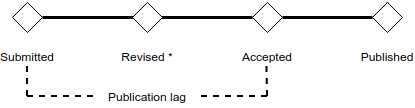
\includegraphics[width=9cm]{images/timeline.drawio.png}
\caption{Milestones in timeline publication model with publication lag}
\label{fig:timeline}
\end{figure}

From this process we can measure the time between submission and acceptance (
publication-lag) and use this measure as comparison with other authors en within 
the same venue. A low publication-lag compared with 'normal' can be used to 
identify interesting cases like an abnormal short time of review.

\paragraph{Beneign alternatives}
The possibility exists that a paper is that good, no revision is needed and the 
review did not take that much time. This also results in a low publication-lag.

% ------------------------------------------------------------------------------
\subsection{Member of the editorial board is (co-)author}
In this case, publications in a venue are co-authored by a member of the 
editorial board, which means he is publishing his own work. A questionable case
in this situation is Griffiths\footnote{\url{http://deevybee.blogspot.com/2020/07/percent-by-most-prolific-author-score.html}}.
Except for editorial boards, this can also happen for conferences.
In Figure~\ref{fig:eia} we present an instance model of this situation.
\begin{figure}[H]
\centering
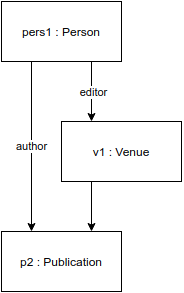
\includegraphics[width=3cm]{images/editor_is_author.drawio.png}
\caption{Instance model of the situation where the editor is (co-)author of the publication}
\label{fig:eia}
\end{figure}


\paragraph{Attack}
We can imagine a situation where the author is being forces to mention the 
person-of-interest as co-author. Which is abuse of the power of the editor.

\paragraph{Model impact}
The impact on the publication model is between the person which is editor for a 
venue, and the venue itself. 
The number of publications he has in that venue while he works for that venue 
will increase. For detection we can measure how much he publish in the Venue 
when he work for that specific venue.
One metric we need here is \textit{number\_of\_publications}. Also with the case~\ref{sec:work_member_editorial_board_cited}, we need the number of issues 
here.

% ------------------------------------------------------------------------------
\paragraph{Beneign alternatives}
Besides possible ethical questions that can be raised, there is a perfectly good
reason for someone to publish in the venue he is editing. Say, a person is a 
specialist in his field and works at a venue which publishes about this 
specific subject. He has new work to publish but there is not another venue 
which captures this subject.


% ------------------------------------------------------------------------------
\subsection{All time favourite: Diederik Stapel}
\outline{ergens in het begin: er zijn manieren om te frauderen...}

The fraud that Diederik Stapel committed was not related to the publication 
process, but to the data he used to draw conclusion on.
With our specific method, we will not be able to detect data manupulation and
fabrication.

\outline{door neven effect van fraude (bijvoorbeeld heel veel publicaties) of zijn resultatenn halen het nieuws / opgemerkt in academische wereld omdat ze fout zijn / omdat heel veel citaties eerste maanden zijn}.

% ------------------------------------------------------------------------------

\outline{
\section{placeholder}

\begin{itemize}
    \item Author and reviewer are the same person: $\{h \in \Humans \mid \authors(p, h) \land \reviews(p, h)\}$ (Moon)
    \item Editor-in-Chief is part of authors: $\{h \in \Humans \mid \authors(p, h) \land \receives(p, h)\}$. Logisch gevolg is dus dat $\accepts(p, h)$
    \item Citaat naar paper van iemand in het proces: stel q is de publicatie waar het om draait dan:
    $\{h \in \Editors \cup \Reviewers \mid \cites(q, p) \land \authors(h, p)\}$
    \item bovengemiddeld zelfcitaties
    \item publicaties die geciteerd worden komen uit dezelfde journal\todo{???}
\end{itemize}
}

\outline{
\begin{itemize}
    \item dan modellering (hfst \ref{chp:modelling_the_publication_process})
\end{itemize}
}

% ==============================================================================
\chapter{Related work}
% ==============================================================================
\outline{
Bijdrage aan contributies
\begin{itemize}
    \item 1) Studies die iets soortgelijks hebben gedaan
    \begin{itemize}
        \item Tielenburg
    \end{itemize}
    \item 2) Bouwstenen
    \begin{itemize}
        \item PDF Extractie
        \item Outlier detectie
    \end{itemize}
    \item 3) Titels die altijd moeten worden genoemd
\end{itemize}
}


% ==============================================================================
\chapter{Methodology}
% ==============================================================================
Belangrijkste punten:
\outline{
\begin{itemize}
    \item Wat ga je doen?
    \item Waarom ga je dat zo doen?
\end{itemize}
\begin{itemize}
    \item Draait om detecteren of er aanvallen plaats vinden
    \item Wat hebben we nodig om aanvallen te detecteren (hoe kunnen wij dat 
    doen?
    \item Redenering dat we een model nodig hebben
\end{itemize}
}

% ==============================================================================
\chapter{Modelling the publication process}
\label{chp:modelling_the_publication_process}
% ==============================================================================



\section{Generic Model}

Jonker and Mauw formalised the publication model~\cite{JM2017} and created an entity based \todo{high over view}. Figure~\ref{fig:jm2017_induced_pub_model} depicts their final model, 
which unifies different representations of the same author/paper/venue.
\begin{figure}[H]
\centering
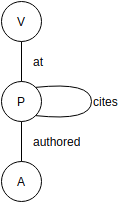
\includegraphics[width=3cm]{images/jm2017_undiced_pub_view.drawio.png}
\caption{Set-theoretic publication model of papers (P), venues (V), and authors (A) (adapted from~\cite{JM2017})}
\label{fig:jm2017_induced_pub_model}
\end{figure}
In this figure, the V stands for venue, P for publication and A for author. Based on this model, research is conducted to identify if interesting authors can be identified based on metrics derived from this model. One such research is the work of Tielenburg~\cite{TEJ2017}. Unfortunately, the results where not sufficient to provide a solid framework to detect interesting authors.



Whereas the Jonker and Mauw only modelled the Author as a role in the process, we can now also get the publisher, editor and reviewer from Bjork and Hedlund. We consider the Author from Jonker and Mauw the same as the Researcher form Bjork and Hedlund.

\todo{Hier moet nog iets meer. Bijvoorbeeld: https://www.councilscienceeditors.org/resource-library/editorial-policies/white-paper-on-publication-ethics/2-1-editor-roles-and-responsibilities/}
\outline{We think it is save to ignore the publisher as a role. The publisher is responsible in the end and sets the regulations and constraints for editors to work within, but the actual work is delegated to editors.}

Unfortunately, Bjork and Hedmung lacks the opportunity to describe the process. However, we can get some textual information from Cormode from his work as an associate editor~\cite{C2013}.

Cormode also focusses on the journal publication. We will gather the roles and responsibilities from his article and use this to complete our perspective.
\paragraph{Editorial Board} Cormode describes that the structure can vary depending per journal. In most cases, generic structure for a journal is that there is a editorial board. This board consist of the Editor-in-Chief and multiple Associate Editors. The main role of this board is to determine which papers to accept.
\paragraph{Editor-in-chief} This role decides which papers to include. The information to make this decision comes from the Associate Editor. This role receives the actual papers and delegate the work to associate editors.


\paragraph{What about the author}
Cormode also gives suggestions to certain roles in the process. In our case, the suggestions he makes for an author are important: 1) Suggest suitable Associate Editor and 2) Suggest suitable Reviewer. If the editor-in-chief and associate editor make use of this suggestion, the author can gain power in the judgement of his own work.



\outline{
\begin{itemize}
    \item Reviews
    \item vaak meerdere
    \item daarom minder risico op fraude???
    \item ali \& watson bekijken
\end{itemize}
}

\section{Extending the model}
The main questions we want to ask are which entities and which roles are involved and how are they related.
To recap, Figure~\ref{fig:jm2017_induced_pub_model} shows the publication model as seen by Jonker and Mauw. We can extend this with the description of Cormode to come up with a model that incorporates the most important roles with influence on the judgement of the work of an author, which results in judgement of the production of the author, which eventual lead to possible the benefits for the author. We ignore roles like the editorial assistance and subeditor, because these roles does not seem to have influence on the judgement of a menuscript. In Figure~\ref{fig:structure_journal} we provide an overview of the entities and roles from Jonker and Maauw combined with the information from Cormode which answers which roles are involved and how they are related.

The red rectangles are objects and the green circles are roles.
As objects we have a venue which contains papers. Multiple roles are related to these objects.
We define the following sets:
\begin{itemize}
    \item Authors: $A(p) = \{h \in H \mid \authors(p, h)\}$
    \item Reviewers: $R(p) = \{h \in H \mid \reviews(p, h)\}$
    
\end{itemize}



\todo{
\outline{
\begin{itemize}
    \item wie kiest de EiC?
    \item Ik lees overal dat deze vaak gekozen wordt uit de editors.
    \item Je wordt editor door vaak en veel te reviewen of als author voor dat journal te werken.
    \item Uiteindelijk wordt je dan gevraagd (KUNNEN WIJ DIT TERUGVINDEN IN DE DATA? (openemen in interessante gevallen?) WORDT MEN ECHT GEKOZEN OP BEWEZEN DIENSTEN? AANSLUITING MET SNCMBL2021???).
    \item Punt is dat je gevraagd wordt als EA (DOOR WIE DAN?) en gekozen wordt als EiC (DOOR WIE? OP WELKE CRITERIA? MOGELIJKHEID TOT VRIENDJESPOLITIEK?).
    \item Ik kan hier niet veel informatie over vinden.
\end{itemize}
}
}

HOE VERDER???
\begin{itemize}
    \item Vanuit fraude oogpunt interessante gevallen / OOK BESTAANDE AANVALLEN???
    \item Voor detectie moeten we data hebben
    \item Welke data is wel beschikbaar / welke niet
    \item Hoe komen we hier aan -> overgang naar hoofdstuk data acquisition
\end{itemize}


% ==============================================================================

\begin{figure}[htbp]
  \begin{center}
  \small
        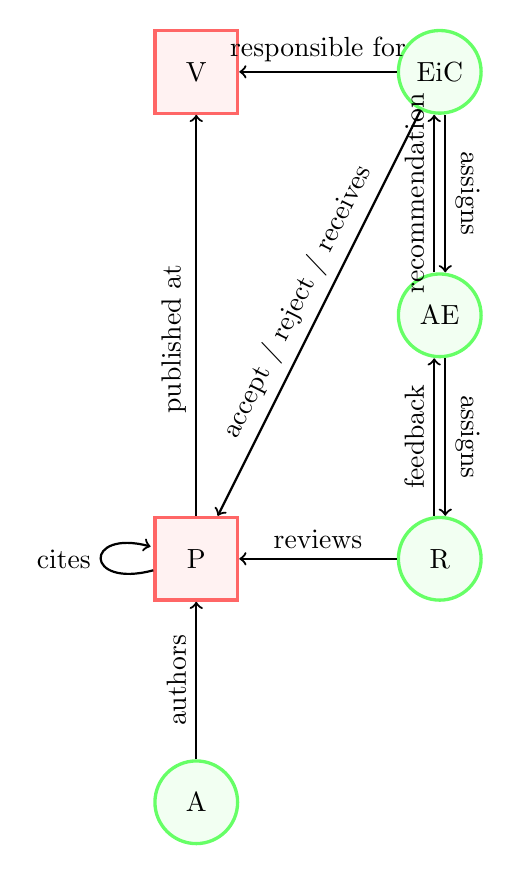
\begin{tikzpicture}[
            auto,node distance=2cm,thick,
            rolenode/.style={circle, draw=green!60, fill=green!5, very thick, minimum size=1.05cm},
            thingnode/.style={rectangle, draw=red!60, fill=red!5, very thick, minimum size=1.05cm},
            ]
            % Nodes
            \node[rolenode] (eic) {EiC};
            \node[rolenode] (ae) [below=of eic] {AE};
            \node[rolenode] (reviewer) [below=of ae] {R};
            
            \node[thingnode] (venue) [left=of eic] {V};
            \node[thingnode] (publication) [left=of reviewer] {P};
            \node[rolenode] (author) [below=of publication] {A};
            
            % Lines
            \draw[->] (publication) -- node [text width=2.5cm,midway,above,sloped] {published at} (venue);
            \draw[->] (eic) -- node [midway,above,sloped] {responsible for} (venue);
            \draw[->] (eic) -- node [midway,above,sloped] {accept / reject / receives} (publication);
            \draw[->] (reviewer) -- node [text width=2.5cm,midway,above,align=center] {reviews} (publication);
            \draw[->] (author) -- node [midway,above,sloped] {authors} (publication);
            \draw[->, transform canvas={xshift=2pt}] (eic) -- node [midway,above,sloped] {assigns} (ae);
            \draw[->, transform canvas={xshift=-2pt}] (ae) -- node [midway,above,sloped] {recommendation} (eic);
            \draw[->, transform canvas={xshift=2pt}] (ae) -- node [midway,above,sloped] {assigns} (reviewer);
            \draw[->, transform canvas={xshift=-2pt}] (reviewer) -- node [midway,above,sloped] {feedback} (ae);
            
            \path (publication) edge [loop left] node {cites} (publication);
            
            % \draw[->] (publication.west) .. controls +(down:7mm) and +(left:5cm) .. (publication.west);
        \end{tikzpicture}
  \end{center}
  \caption{Set-theoretic model of the publication process for collections.}
  \label{fig:structure_journal}
\end{figure}


% ==============================================================================
% \subsection{Roles in the editorial process}
% In the editorial process multiple roles are involved. These roles are executed
% by persons. We define all persons involved somehow in the editorial process by 
% \textit{H}. Publications are defined by the letter \textit{P}.
% % ------------------------------------------------------------------------------
% \paragraph{Author}
% \begin{itemize}
%     \item How evident, this role writes the text to be published.
%     The main question is, how is someone with this role able to influence the process in his favor.
%     One way is to suggest a reviewer and indicate non-preferred reviewers \cite{C2013}. This relates to the case of Moon.
%     \item Suggest Associate Editor
% \end{itemize}
% We define the collection authors of a paper $A(p) = \{h \in H \mid \authors(p, h)\}$

% % ------------------------------------------------------------------------------
% \paragraph{Editor-in-chief}
% Wie bepaalt wie de editor-in-chief is? -> macht
% \begin{itemize}
%     \item receives the manuscript $\receives(p, h)$
%     \item Performs initial check (relevance, suitability to undergo peer review)
%     \item Assigns Associate Editor based on Area of expertise and avoiding potential conflicts of interest between author and AE
%     \item end decision if paper is being published: Stel h = Editor in chief en p = publication dan: $\accepts(p, h)$ of $\rejects(p, h)$
%     \item An editor-in-chief has this role for a certain period (span multiple issues).
% \end{itemize}


% % ------------------------------------------------------------------------------
% \paragraph{Editorial assistance}
% \begin{itemize}
%     \item Checks similarity to other publication (iThenticate)
%     \item Verder geen invloed op process
% \end{itemize}

% % ------------------------------------------------------------------------------
% \paragraph{Reviewer}
% \begin{itemize}
%     \item Reviews a paper
% \end{itemize}
% We define the collection reviewers of a paper $R(p) = \{h \in H | reviews(p, h)\}$
% % ------------------------------------------------------------------------------
% \paragraph{Subeditor}
% \begin{itemize}
%     \item Niet echt relevant
%     \item Om tekst leesbaarder te maken
% \end{itemize}
% % ------------------------------------------------------------------------------
% \paragraph{Associate editor}
% \begin{itemize}
%     \item Identify and Assigns reviewers
%     \item administrative reject (desk reject): vaak al in eerder stadum eruit 
%         gehaald door Editor-in-Chief of Editorial assistance
%     \item recommendation to editor in chief
%     \item Following roles sometimes combined into the Associate Editor:
%     \item Managing editor
%     \begin{itemize}
%         \item Checks journal standards, word length, use of internal reporting 
%             standard
%         \item assigns editor
%         \item assigns reviewers
%     \end{itemize}
%     \item Editor
%     \begin{itemize}
%         \item Initial check
%     \end{itemize}
%     \item This role is also for a period of time
% \end{itemize}
% ------------------------------------------------------------------------------





% ==============================================================================
\section{General process}
Bjorn and hedlund descirbed the publication process from a cost perspective 
\cite{BH2004}. We can use this to visualize the publication process from a time 
perspective. This view is input to determine if we are able to collect all 
necessary metrics.



% ==============================================================================
\section{Flow proceedings and conferences}


% ==============================================================================
\chapter{Group identification}
% ==============================================================================
The first step in detecting outliers is to identify groups of people who are in 
the same position. We identify the followig groups in his research because they
may be interesting.

\section{Editors of proceedings}

\section{Authors submitting at the same conference}

\section{Author submitting at the same journal}

\section{Authors that publish with each other}

\section{H-Index}


% ==============================================================================
\chapter{Extracting auxiliary publication data}
% ==============================================================================
\begin{itemize}
    \item There is more to the publication process than the data
        in A-miner / DBLP can tell you.
    \item Examples: PC memberships, editorships, reviewers (who reviewed which paper),
        how fast was the review process, etc.
    \item Some of this data is publicly available, but not integrated into existing
        publication data sets.
    \item For example: Elsevier gives timelines of paper revisions for journal articles;
        in their LNCS series, Springer typically lists the PC members in the front matter.
    \item This data may be useful for identifying outliers.
    \item In this chapter, we investigate how to extract both Elsevier and LNCS data and
        how to integrate them with existing data sources.
    \item
    \item 
    \item People involved in the proceedings are mentioned in the Front Matter.
    \item Front Matter can be downloaded as PDF.
    \item PDF are considered unstructured data.
    \item PDF's are meant to read by humans, not computers. However, currently 
        we have 4370 Front Matters, which is an unbearable task to copy and 
        paste the data manual from these PDF's.
    \item To be able to get the data inside these PDF's, we need to convert the 
        PDF's to a structured or semi-structured dataset.
\end{itemize}

\section{Reading a PDF}
\begin{itemize}
    \item Multiple options to make the pdf computer-readable:
    \begin{description}
        \item[Convert to HTML] There are multiple tools available to convert PDF
            to html format. Further processing can be applied by using HTML
            libraries. Unfortunately, this HTML pages are complex to interpret
            because a tag can contain just one letter. We need to glue these 
            tags together, with taking the location of the tag in consideration
            (how much space is between two letters, is that a space, is that a 
            new column, or an indent in an existing column etc.). We did an 
            experiment to process PDF's this way, but the resulting solution to 
            process one PDF was not able to process another one. The effort to 
            make this a generic solution which can easily be extended where 
            necessary was very high in comparison with the result we achieved.

        \item[Convert to plain text] Almost all libraries to read a pdf file 
            support the option to read the file as plain text. Drawback is that
            the lay-out is gone. This lay-out is necessary to get some structure
            from the document.
        
        \item[Convert to image and extract text] This was we can use machine 
            learning liberaries to get the text from an image. We tries this 
            with Tesseract, but too much information was lost to get the 
            structure of the document.

        \item[Use low level library] In this experiment we tried of we were able
            to process the PDF with a more low level library. This give us more
            control of the process. First small experiments with PDFBox were 
            succesfull.
    \end{description}
\end{itemize}

\section{A prototype extractor of raw data}
\todo{We chose option 4 because \$REASONS.}
\begin{itemize}
    \item First we need to get the raw data from the PDF's.
    \item PDFBox has an parser that gives the PDF back as text. As mentioned
        before, for our case this is not enough. The problem is within this text
        all spaces between words are converted to one space. However, we need to
        be able to identify columns, so we need to keep all spaces.
    \item Luckely, we were not the only one with this problem. On 
        Github\footnote{\url{https://github.com/JonathanLink/PDFLayoutTextStripper}} 
        there is an open source additional parser available for PDFBox that 
        keeps the layout as is.
    \item However, this extension still did not have all properties of a text we
        need to get the structure of a file. Luckely, because this extension 
        issue open source, we can add this information to the text objects we 
        read from the PDF.
    \item Besides the text with all the spaces in between we get by using this 
        extension, we also added:
    \begin{itemize}
        \item FontSize
        \item FontSizeInPt
        \item XScale
        \item IsBold
    \end{itemize}
    \item The result is now that we have the pdf file as textobjects with 
        extra properties.
\end{itemize}

\subsection{Building a document tree}
\label{sec:lncs_parser_doc_tree}
\begin{itemize}
    \item By using the properties textsize and bold we are able to build an 
        hierarchical structure of the document. 
    \item We need this, because in most
        Front Matters there is an organization header, with subheaders 
        containing the role of the people.
    \item As datastructure to work with the data we use a tree.
    \item The objects we store in this tree are Sections. These contain the 
        textlines and the header as title of the section.
\end{itemize}

\subsection{Focus on organisation}
\begin{itemize}
    \item Having this tree, we can easily get the section that contains the 
        organisation (because this section is called, you have never guessed it, 
        'organisation').
    \item Because we have a tree data structure, we can ask this organisation 
        section to loop trough all sections underneath.
\end{itemize}

\subsection{Processing a section}
\begin{itemize}
    \item All text in a section that is under a role, has some kind of table 
        struture.
    \item For that reason we use a grid a data structure to put the data from 
        the raw lines in to.
    \item This grid structure gives us some possibilities, e.g. to get 
        statistics of a column.
    \item The challende in this part is to merge lines into one line.
    \item This process is done in a section to grid converter. To separate this
        process from the process of building a tree, improves testability.
\end{itemize}

\subsection{Getting information from a grid}
\begin{itemize}
    \item We calculate some statistics of a grid which we need to choose a
        parser further down the processing.
    \item The statistics we get:
    \begin{description}
        \item[Number of textparts] The total number of cells that are filled in
            the grid.
        \item[Number of columns] The number of columns that the grid contains.
            Most sections contains two columns, but this is certainly not the 
            case for all sections.
        \item[Affiliation ratio] The ratio of textparts that contain keywords 
            for an affiliation (e.g. "universi"). This is calculated for every 
            column and for odd, even and all rows.
        \item[Comma ratio] Same as affiliation ratio, but for comma's. Can also
            be used to identify affiliations. However, names also contains 
            comma's if the format is lastname, firstname.
    \end{description}
    \item All this information is stored in a SectionInfo object which is added
        to the section.
\end{itemize}

\subsection{Choosing a parser}
\begin{itemize}
    \item With the information the program can choose the appropiate parser to
        interpret the data correctly and convert the grid into members.
\end{itemize}

\section{Data storage}
\begin{itemize}
    \item During this process we store data in a database and in logfiles.
\end{itemize}

\subsection{Database}
In the database we store three entities: file, section and member. All tables 
contain at least the following attributes:
\begin{description}
    \item[id] Auto generated number.
    \item[run\_id] The identification of the program run (epoch).
\end{description}
In Figure~\ref{fig:lncs_pdf_database} the relationship between the tables are
shown.
\begin{figure}[H]
    \centering
    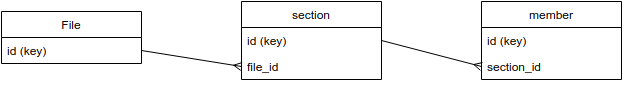
\includegraphics[width=12cm]{images/lncs_pdf_parser_tool.drawio.png}
    \caption{Relationship between tables}
    \label{fig:lncs_pdf_database}
\end{figure}

\subsubsection{File}
This table contains information of the file. It can be use to link to previous 
gathered data. The following attributes are in this table:
\begin{description}
    \item[filename] The filename of the pdf to refer to other tables in the 
        process.
    \item[status] If the process of the file succeeded or failed.
    \item[message] If the process failed, how come. 
\end{description}

\subsubsection{section}
This table contains information of the section. The following attributes are in 
this table:
\begin{description}
    \item[title] The title of the section (e.g. Program chair).
    \item[num\_parts] The number of textparts that are detected in this section.
    \item[num\_section\_lines] The total number of lines in a section.
    \item[num\_section\_lines\_non\_empty] The number of lines in a section that
        are not empty.
    \item[num\_merges\_lines] The number of lines that are merged in to the 
        previous line.
    \item[num\_grid\_rows] The number of rows the grid has.
    \item[num\_grid\_columns] The nubmber of columns the grid has.
    \item[all\_values\_contain\_commas] Indicator if all values contain commas.
    \item[comma\_ratios] A json structure with statistics of comma's in the text.
    \item[affiliation\_ratios] A json structure with statistics of affiliation 
        keywords in the text.
    \item[parser] The parse the program choose to process the section.
\end{description}

\subsubsection{Member}
This table contains eventually the resulting data we are interested in.
\begin{description}
    \item[role] The role of the member. This is in most cases the same as the 
        the title of the section (but, not always). 
    \item[name] The name as we get from the data, whatever format it is. If we
        get a separate firstname and lastname from the section, the name is 
        built based on those values. However, we prefer separate firstname and
        lastname, because this gives us more options when we need to integrate
        this data with data from other sources.
    \item[firstname] If we are able to get separate firstname and lastname of
        the member, we will store this here. We do tend to interpret names which 
        contain a comma as <lastname>, <firstname>.
    \item[lastname] Same as before, but then the lastname :).
    \item[affiliation] The affiliation of the member. This data is not always
        available, but we do not tend to use it.
\end{description}

\subsection{Iterative Logging-based development process}
For every file that the program process, it keeps a separate logfile. This gives
us the ability to investigate why the program was unable to process some files 
or sections. Missing parser for example can be detected using this mechanism in
combination with the data in the section table in the database.

For every file the logfile shows the document tree as described in 
Section~\ref{sec:lncs_parser_doc_tree}. 

If sections are found, the logfile shows for every section:
\begin{description}
    \item[Textlines] All the lines that are in this section.
    \item[Grid] The derived grid from the textlines.
    \item[Members] The members that are extracted from the section.
\end{description}
This may seem a lot, but having this information gives us the possibility to 
investigate in detail why data can not be interpreted and easily build new 
functionality (e.g. new parsers) and add unit tests for this functionality.

\section{Validation}
Currently 4370 Front Matters are available. How are we able to tell something 
about the quality of the program without manually go through the results?

For every section we have some metrics. With these metrics, depending on the
parser we can see if the number of extracted members is correct, or close to
correct.

For example, The parser Two\_Role\_NameAff contains two columns: first with a name
and second with the affiliation. We can measure if the number of resulting 
members is equal to the non-empty lines in the section minus the merged lines.



\subsubsection{Current state}


\begin{figure}[H]
    \centering
    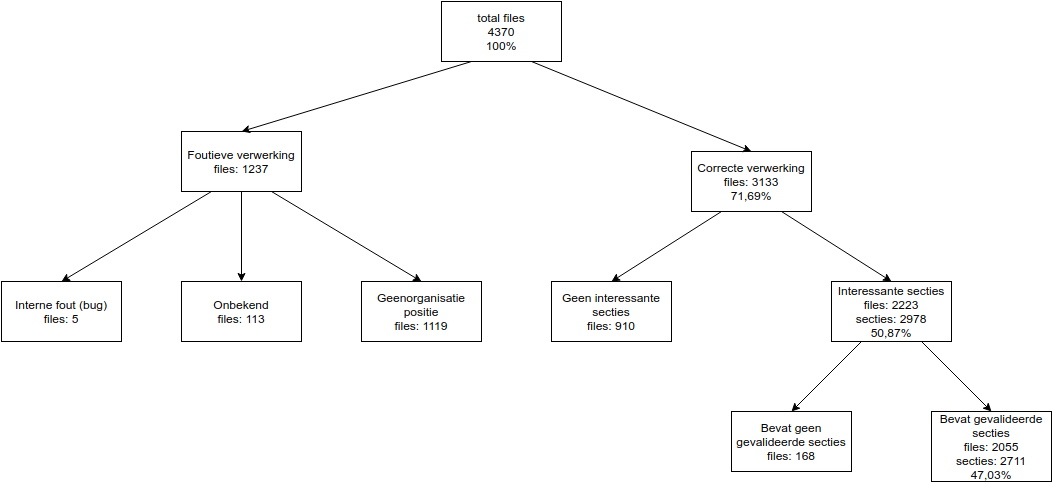
\includegraphics[width=17cm]{images/lncs_front_matter_result.drawio.png}
    \caption{Current results}
    \label{fig:lncs_pdf_database}
\end{figure}


% ==============================================================================
\chapter{Data integration}
% ==============================================================================
To get an integrated dataset across all sources some challenges need to be 
addressed. Also, to be able to integrate the sources where we need to get the
data from, we sometimes need to get data from another source.

The main entities we need to integrate are person (authors, members of program
committees etc.) and articles (chapters from lncs with papers from aminers).

\section{Integration of persons}

First challenge is to make the authors unique. This comes with the
second challenge of data quality.

For example, from springer we scrape get the chapters (inproceedings) and their 
authors from their site. This authors sometimes comes with an orcid, which 
should be unique. However, we found situations where an author gets an orcid of
someone else. This is a data quality issue.
\todo{voorbeeld toevoegen}
Luckely, this does not occur much, and for the few it occurs we can easily 
create a manual file to override this. Of course with caution; if two orcid 
have the same name, we can not override this; some authors have the same name.
On the other hand, if one orcid refers to a totally different name, we can.


Seconds challenge is that a name does not make an author unique. The same name
refers to other authors. Luckely, DBLP addresses this problem by suffixing the
name with a four digit code~\footnote{\url{https://dblp.org/faq/1474704.html}}.
DBLP is making progress here, but this is not entirely done yet. But even if
they mention to unique identity authors, the match to authors in other 
datasources (like Aminer and Springer) is not straightforward. In that case we 
need to ignore the authors from these sources and make the match by going 
through the paper (or chapter, as is it is called within LNCS Springer).

Third challenge is the name. For most authors these sources do not contain an
orcid or an email address, which means we need to match the authors on name.
But, in some sources the names are fully written (with or without the 
middlename), sometimes the middlename only has a initial while the firstname is 
fully written, and sometimes we only get the initials and lastname.
DBLP covers this by naming all aliases of a single person.

Still we do have a problem, because inthe end we need to match these authors
with members we get from the frontmatters of lncs. Within this frontmatters, 
there is no orcid, email, or a four digit number to match to dblp records; these
documents or not written with the intention to identify persons.

\subsection{Approach}
\begin{itemize}
    \item Get DBLP data dump and create unique authors. DBLP also has their 
        aliases and sometimes orcid.
    \item Also use this dump to get the inproceedings, incollections and 
        articles.
    \item This dump can also be used to create the author relationship between 
        articles and persons.
    \item Integrate springer lncs chapters into the article entity.
    \item Use springer lncs to get the book (collection) and identify the 
        relationship between chapter and book.
    \item Integrate members from the frontmatter into the person entity.
    \item Use he frontmatter to lay the relationship between the proceeding and
        the person.
    \item *** Now we can get a few groups
    \item Integrate the aminer papers in the article entity.
    \item Use aminer to get the relationship between articles.
\end{itemize}

\section{Integration of papers}

So, the next issue then is how we can match the papers. In this case we can use
the document id. However, this document id is not filled in for all titles. For
the papers that do not have an doi, we can do the match on title. Unfortunately,
this also is not that straightforward. The title sometimes contains latex 
specific characters, or other weird characters.
\todo{voorbeeld toevoegen}

To get the groups we identified, we need to integrate the chapters from lncs 
frontmatter with the papers from aminer.

% ==============================================================================
\chapter{Data acquisition}
% ==============================================================================
\outline{
\begin{itemize}
    \item Question to answer: Which data do we need and how can we get it?
    \item om te weten welke data we nodig hebben kijken we naar het publicatie process -> beschreven in voorgaand hoofdstuk
    \item vervolgens kijken we naar de data die beschikbaar is in de publiek beschikbare databronnen
    \item mismatch
    \begin{itemize}
        \item welke informatie missen we
        \item hoe kunnen we hier aan komen
    \end{itemize}
    \item ophalen van mismatch
\end{itemize}
\begin{itemize}
    \item Publicly available sources are limited in available data. Most datasets provides information on who wrote what and sometimes which article refers what. This provides a good insight and based on these datasets a lot of research is already conducted.
    \item However, we think these datasets miss actors on the publication process that are in a position with enough power to influence the publication process.
    \item Data about these people involved in the publication process are not structured available to use in analysis. The information is provided in front matters and masthead documents. Because of the nature of these documents, mostly PDF's, we consider this as unstructured data.
    \item We are somehow surprised of the lack of structured data availability about these people, because of their power and influence.
    \item Our focus in this chapter is to incorporate this less structured available data into publicly available data about the publication process to get a dataset which provides a more complete view of the publication process.
    \item Our research focus on information technology so our start point to gather these people is to use the most prominent conferences and journals. As source for this data we use the core ranking.
\end{itemize}
}

\subsection{Editorial board}
\begin{itemize}
    \item Editor-in-chiefs, associate-editors and sometimes a list of reviewers (generic, not who reviewed what paper) are most of the time available on the publisher of the specific venue. 
    \item This is a positive point.
    \item However, this is most of the time not machine readable (which is; easy to query through an interface). It is placed on the website for humans to read.
    \item The second issue is that only the current editorial board is shown on the website. This may be sufficient for guest of the site, but for collection data with the purpose of detecting fraud, this is not sufficient.
    \item Not everything is lost however; Most of the time the previous editorial boards are available in mastheads of a certain issue. Most of the time written in PDF's (as chapter in the journal). Also within one publisher, the format in which these mastheads are presented changes.
    \item The combination of the facts above make it hard for a fraud detection system to use this information.
    \item These are known fraud cases where this information is worth to have:
    
\end{itemize}

\subsection{publication lag}
\begin{figure}[H]
\centering

\includegraphics[width=5cm]{ACM_Digital_Threats_Research_and_Practice.png}
\caption{Publication history of an article in ACM (\url{https://dl.acm.org/doi/10.1145/3442445})}
\label{fig:acm_dates}
\end{figure}
\begin{itemize}
    \item A paper goes through certain stages until it is published.
    \item Not all publishers expose the dates these stages are achieved. 
    \item Fortunately some do. For example ACM (\ref{fig:acm_dates}) and Springer. However, this is not for all publications available. So there are some missing data points.
    \item Fraud cases where this information can be helpful:
    \begin{itemize}
        \item Moon was detected because the time that his work was submitted and was approved by the reviewer (which was Moon himself) was remarkable short.
        \item ~\cite{SNCMBL2021}
    \end{itemize}
\end{itemize}

\section{Public available datasets}

\outline{
\begin{itemize}
    \item Model wat in dblp, aminer en in HJ staat
    \item Model publicatieprocess
    \item Sluit niet aan
    \item meer rollen -> niet in publieke datasets
    \item Most public available datasources for the publicationprocess contain information about the author and what the author publices. Sometimes (but not all, or incomplete) these datasets also contain references.
    \item The model of these datasets are visualized by the publication process of Jonker and Mauw.
    \item Examples of these datasets are DBLP and Aminer.
\end{itemize}
}



\subsection{DBLP}

\begin{figure}[H]
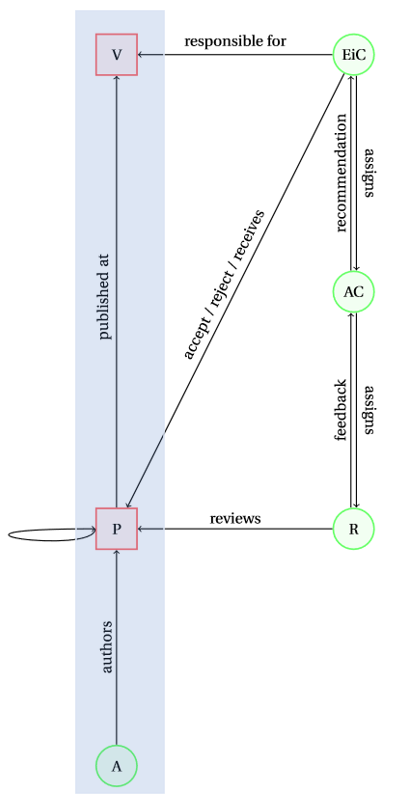
\includegraphics[width=5cm]{incollection_dblp}
\centering
\caption{In Collection DBLP}
\end{figure}

\outline{
\begin{itemize}
    \item Wat is DBLP
    \begin{itemize}
        \item DBLP is a dataset with information about publication in the computer science discipline.
        \item 
        \item Transformed to relational tables.
        \item Result is 35 tables.
    \end{itemize}

    \item Structure of delivery
    \begin{itemize}
        \item Datastructure of DBLP is XML.
        \item contains bibliographic records; like example
        \item These bilbiographic records have elements such as author, title, journal
    \end{itemize}
    \item Processing
    \begin{itemize}
        \item convert XML to relational tables
        \item Every bibliographic type in separate table
        \item Assign unique id
        \item Make separate table for elements with id of bibliographic record
        \item Attributes of elements are columns in table
        \item Add metadata to all data entries
    \end{itemize}
    \item Result
    \begin{itemize}
        \item 35 tables
        \item overzicht van tabellen en relaties
    \end{itemize}
\end{itemize}    
}


\lstset{language=XML}
\begin{lstlisting}[caption={DBLP bibliografic record example},label={lst:DblpExample}]
<article mdate="2019-10-25" key="tr/gte/TM-0332-11-90-165" publtype="informal">
<author>Frank Manola</author>
<author>Mark F. Hornick</author>
<author>Alejandro P. Buchmann</author>
<title>Object Data Model Facilities for Multimedia Data Types.</title>
<journal>GTE Laboratories Incorporated</journal>
<volume>TM-0332-11-90-165</volume>
<month>December</month>
<year>1990</year>
<url>db/journals/gtelab/index.html#TM-0332-11-90-165</url>
</article>
\end{lstlisting}
\begin{itemize}
    \item Bibliografische records zijn gedefinieerd door een element met subelementen. Deze subelementen bevatten waardes, en geen andere elementen.
    
    \item 
    \begin{itemize}
        \item zie author element in voorbeeld
        \item moeten manier vinden om hier mee om te gaan
        \item oplossing is id generereren voor elk 'parent' object.
        \item dit zijn objecten die direct onder de tag <dblp> vallen.
    \end{itemize}
   
    
    
    \item deze objecten aparte tabellen opslaan
    \item waarbij tabel naam de naam van het attribuut is (bijv. article)
     \item ander probleem geen zuivere xml: 
    \lstset{language=XML}
    \begin{lstlisting}[caption={XML fout},label={lst:DblpExample2}]
    <title>Graphs of Bounded Treewidth can be Canonized in AC<sup>1</sup>.</title>
    \end{lstlisting}
    
\end{itemize}

\subsection{Aminer}

\begin{figure}[H]
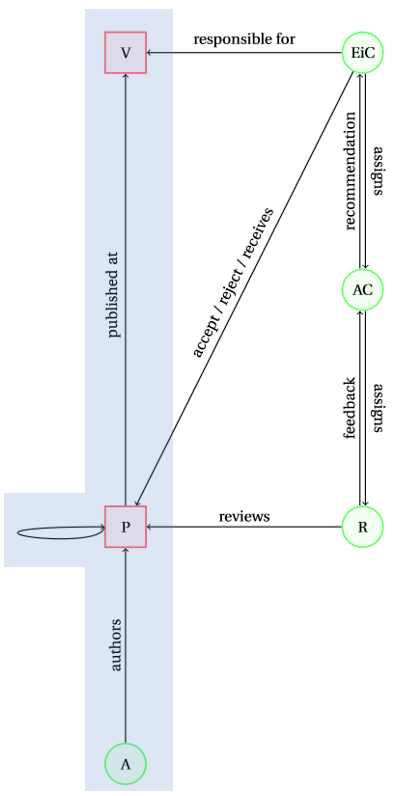
\includegraphics[width=5cm]{incollection_aminer}
\centering
\caption{In Collection DBLP}
\end{figure}

\section{Deviation publication model and available data}
\begin{itemize}
    \item Publicatieprocess sluit niet aan met beschikbare databronnen
    \item We missen het volgende:
    \begin{itemize}
        \item dit
        \item dat
        \item zus
    \end{itemize}
\end{itemize}

\section{Overcoming the difference}
\begin{itemize}
    \item Tielemans vooral gebasseerd op beschikbare data (DBLP)
    \item Machtsverhoudingen komen niet terug in de publieke datasets
\end{itemize}
\subsection{Justification}
\begin{itemize}
    \item Overzicht real-life cases (probleem verder beschrijven)
    \begin{itemize}
        \item Voorbeeld Vasilakos, citaten uit 2 journals waar hij zelf in zit
        \item Publicatie lag
    \end{itemize}

\end{itemize}
\subsection{Process and choices}
\subsection{Case study: Lecture Notes in Computer Science}
\outline{
\begin{itemize}
    \item dat je ze krijgt niet interessant
    \item wel waarom, en hoe goed
\end{itemize}
}

\subsection{Case study: Publication lag}

\section{Conclusion}
\outline{
Antwoord op welke data is nodig en hoe komen we eraan

}

% ==============================================================================
\chapter{Data integration}
% ==============================================================================
\outline{
    \begin{itemize}
        \item Three main sets to intergrate: Humans, Venues, Publications
    \end{itemize}
    \section{Publication}
    \begin{itemize}
        \item Root is DBLP
        \item Key is DBLP key
        \item We need to integrate the publications from DBLP with Aminer
        \item DBLP is leading, so we need to match publications from dblp to aminer
        \item In two steps: First try to match on DOI, second, match on title
    \end{itemize}
    \subsection{Document Object Identifier}
    \begin{itemize}
        \item Wat is het? DOI is unique identifier of a document
        \item Hoe in DBLP?
            DBLP contains additional information about an entry in an ee tag.
            These contain links to doi.org, wikidata, etc.
            Sometimes an article has multiple doi.org links; this seems to be the case with the publisher ACM.
            Although the links are different, they result in the same page at ACM.
            for articles:
            number of doi, number of articles
            0 -> 322169
            1 -> 1094002
            2 -> 728
            3 -> 61
            most articles do have a link to doi.org in the ee
    \end{itemize} 
    \subsection{Enrichtment of DOI's}
    Some publication do not have an DOI in DBLP, but provide an additional link to arxiv site, or wikidata
    \paragraph{Arxiv}
    \begin{itemize}
        \item Arxiv sometimes has a DOI (but not always).
        \item We extact docuemnt information from the Arxiv API. As we were there, we also extracted the authors.
    \end{itemize}
    \paragraph{Wikidata}
}



\outline{
\begin{itemize}
    \item Onderzoeksvraag: Welke data is nodig en hoe kom je eraan?
    \item Doelstellingen:
    \begin{itemize}
        \item Data verzamelen
        \item Data analyseren
    \end{itemize}
\end{itemize}
}




% % ==============================================================================
% \chapter{Data Acquisition}
% % ==============================================================================
% \outline{


% \outline{


% }

% \section{Our root: Computing Research and Education Association of Australasia ranking}
% \begin{itemize}
%     \item CORE
%     \item Australian based, so might be biased
%     \item A website which ranks conferences and journals
%     \item Ranking is from A* to C. Our focus is for the ranking A*, A and B
%     \item The conference list contains the following attributes:
%     \begin{itemize}
%         \item Title
%         \item Acronym
%         \item Rank
%         \item DBLP link
%     \end{itemize}
% \end{itemize}
% \subsection{Gathering the data}
% \begin{itemize}
%     \item Choices for data acquisition:
%     \begin{itemize}
%         \item Use the export functionality on the website
%         \item Scrape the data from the HTML pages
%     \end{itemize}
%     \subsection{Methods}
%     \paragraph{Export functionality}
%     The core websites offers the functionality to download all the data in a CSV file. This is very useful, because 1) this allows us to get the data in a format that is simple to process in a database (we can consider this a table) and 2) it is fast to get the data.
    
%     The drawback however is that this data does not contain the DBLP url. This means we are not able to find related data in a structured manner.
%     A possible way to work with this problem is to manually add the dblp url's ourselves, but this is a labour intensive job, comes with a cost in reproducability and, because of the manual effort, is error-prone.
    
%     \paragraph{Webscraping}
%     \begin{itemize}
%         \item The core website contains the data in a HTML table accross multiple pages.
%         \item With GET request able to get this -> so we are able to automate this.
%         \item All data that is in the table is at our disposal.
%         \item Also the dblp url in the href of the Anchor tag.
%         \item Drawback: Need to build a script for it, which take more time than simply click the export button.
%     \end{itemize}
    
%     \paragraph{Copy-pasting from the website}
%     \begin{itemize}
%         \item Html table, so easy to paste in a table
%         \item Manual work: not convenient for reproducability
%         \item Also unable to find the DBLP url (we only get the 'view'-text in this case)
%     \end{itemize}
    
%     \paragraph{Method conclusion}
%     \begin{itemize}
%         \item We choose to build a script to scrape the data over downloading the export
%         \item Main reason was reproducability and less error prone in finding the DBLP urls.
%     \end{itemize}
    
%     \subsection{Process}
%     \begin{itemize}
%         \item pagination is given in the url
%         \item While testing the site we discovered that when requesting a page outside the pagination number, we did not get a 200 (OK) response
%         \item Loop through pages untill we do not get a 200 (OK) response
%         \item Get the data from the table
%         \item Write it to database
%         \item build in python because... not really a reason except it's hip and happening (and I honestly don't know why)
        
%     \end{itemize}
    
%     \subsection{Result}
%     \item The result was the data presented in two tables in schema 'core': 1) conf-ranks (conference rankings) and jnl-ranks (journal rankings)
%     \paragraph{Completeness}
%     Core conference data:
%     \begin{itemize}
%         \item 883 rows in total, within scope (because of rank): 486
%         \item No DBLP link for 24 conferences within our ranking focus.
%         \item To get this data we manually looked up the dblp url and added this data to the database. We were able to to find the dblp urls of 17 conferences, which remains 7 unknown
%     \end{itemize}
    
    
%     \item From this point we split the data acquisition process in two lanes:
%     \begin{itemize}
%         \item Conference tracks
%         \item Journal tracks
%     \end{itemize}
    
    
% \end{itemize}


% \section{Conference track}
% \begin{itemize}
%     \item Input is conf-ranks form core combined with manual searched DBLP urls
%     \item Purpose is to get the proceedings of the conferences
%     \item One conferences has one or more proceedings
%     \item DBLP contains this data
% \end{itemize}

% \subsection{Gathering DBLP data}
% \paragraph{Methods}
% \begin{itemize}
%     \item Download DBLP database
%     \begin{itemize}
%         \item Already done in project preparation
%         \item BUT; looking for certain proceedings were not available in download, but do on web
%     \end{itemize}
%     \item Use the API
%     \begin{itemize}
%         \item DBLP offers an API to download information.
%     \end{itemize}
% \end{itemize}
% We used the API to extract the data. Because the data is more complete.

% For all conferences in the core table (combined with some manual adjustment), we extracted the proceedings from DBLP.
% This resulted in 15994 proceedings.

% Looking for the most used publisers:
% \begin{table}[h]
% \begin{tabular}{ll}
% \hline
% Publisher & \# of proceedings \\ \hline
% Springer  & 4674              \\
% ACM       & 4010              \\
% IEEE *    & 3592             
% \end{tabular}
% \end{table}
% *IEEE also includes IEEE Computer Society
% } % END OUTLINE

% \section{PDF Reading}
% \outline{
% \begin{itemize}
%     \item Uitdiepen complexheid PDF extractie
% \end{itemize}
% }
% \begin{itemize}
%     \item PDF is mostly text plotted on a sheet with certain coordinates and properties. (also images, but we are not interested in these)
%     \item options: PDF to html
%     \begin{itemize}
%         \item Problem changed from interpreting PDF to interpreting HTML
%         \item Still need to be able to 'understand' the relationships between certain elements on the page
%     \end{itemize}
%     \item OCR (tesseract)
%     \begin{itemize}
%         \item OCR is a technology to detect characters from images
%         \item PDF is not an image, so first need to convert the PDF's to images
%         \item Output is plain text or TSV. Lot of contect (like position) gets lost in the process. This information is crucial if we want to interpret the pages.
%     \end{itemize}
% \end{itemize}
% \subsection{pdf to html}
% \begin{itemize}
%     \item Volgende libraries geprobeerd:
%     \begin{itemize}
%         \item PDFMiner
%         \begin{itemize}
%             \item Tries to split blocks of text
%             \item can be nice, but in these kind of documents, there is mostly a relation between the columne (like 'person' and an 'affiliation')
%         \end{itemize}
%         \item pdf2htmlex
%         \begin{itemize}
%             \item Most promising
%             \item Lots of CSS
%             \item Spaces can be tricky. Sometimes there is a space, but with a margin class with a negative number, so letter-space minus the margin, becomes so little, we have to ignore this space.
%             \item on the other hand, sometimes there is no space, but the space needs to be derived from the letter-spacing.
%             \item other challenge are items in a column that do not fit the row, so it continues on the next row. How do we consider this text as part of which column?
%         \end{itemize}
%     \end{itemize}
% \end{itemize}
% \subsection{Interpreting HTML}
% \begin{itemize}
%     \item what is the scope of the document we need? For LNCS, Springer provides a template where this section is calles 'Organization'. This is not used in all cases. From whcih point in time did they choose to use this template? Are there other keywords we can use? (like of a lot of subsection headers contain words like 'committee' or 'chair').
%     \item Can we set the scope by interpreting the format? Most of the lists with names are columns.
%     \item When do we consider an element an affiliation? it seems that most (if not all) affiliation have a comma to wplit the country name.
%     \item Can we consider all elements in a column if most of them have a comma as affiliation? No, sometimes names are also <lastname>, <firstname>. But when this is the case, this happens at the first column also, and affiliatons are not likely to be placed in the first column.
% \end{itemize}
% Approach 1: Directly raed HTML elements and see if we can make this work for the LNCS frontmatters.
% \begin{itemize}
%     \item Not sustainable
%     \item hard to maintain
%     \item lots of if-then rules
%     \item good first step to see what is working and what we need to take into account
% \end{itemize}
% Approach 2: First create a model of the HTML document, from this model create a graph with sectionheaders and sections.
% \begin{itemize}
%     \item How to detect section headers? Option; get the font-size that is most used. consider this as the size of the content. Everything that is bigger, assume headers.
% \end{itemize}

% ==============================================================================
\chapter{Data Analysis}
% ==============================================================================
\outline{
\begin{itemize}
    \item Wat betekent de data?
\end{itemize}
}

\section{Validation}
\outline{
\begin{itemize}
    \item Werkt je methode
    \item Aan het eind van ieder hoofdstuk of een eigen hoofdstuk
\end{itemize}
}

% ==============================================================================
\chapter{Conclusions}
% ==============================================================================
\outline{
\begin{itemize}
    \item Samenvatten
    \item Niet alleen samenvatting!
    \item Wat is de impact op de wereld? Wereldvrede :)
    \item Wat zouden we moeten doen en hoe kunnen hiervan profiteren?
    \item Misschien combineren met Discussions?
    \item Voorbeeld discussions
    \begin{itemize}
        \item Op generieke manier wetenschappelijk fraude detecteren, kan dit automatisch?
        \item Misschien meer data
        \item Imago schade als publishers niet meewerken
    \end{itemize}
    \item Misschien combineren met recommendations
    \begin{itemize}
        \item Informatie machine-readable aanleveren
    \end{itemize}
\end{itemize}
\section{Discussion}
One way to decrease fraud in the publication process is to step away from the
current way of judging a researcher. The University of Utrecht is moving to 
another method to judge their researchers based on their effort to promote open
research and their teamwork 
\footnote{\url{https://www.nature.com/articles/d41586-021-01759-5}}. With this 
movement the university is abandoning the indices based on publications and 
citations.
\begin{itemize}
    \item Hoe kan men dan oordelen waar budget heen moet?
    \item Hoe beoordeelt men de toegevoegde waarde van een onderzoeker 
    objectief?
    \item Wat is de impact hier van op de 'piramide'-structuur van 
    universiteiten?
    \item Hoe kunnen medewerkers bij de UU de overstap maken naar een 
    universiteit die beoordelingen wel basseren op impact factor?
    
\end{itemize}
}

% ==============================================================================
\chapter{Recommendations}
% ==============================================================================
\outline {
\paragraph{meer data openbaar maken}
\begin{itemize}
    \item bijvoorbeeld publicatielag
    \item Niet spannend (weinig moeite voor publishers), wel grote verrijking
\end{itemize}
\paragraph{Meer fraud detectie inzetten door publishers}
\begin{itemize}
    \item Kwaliteit van dit stukje van het publicatieprocess borgen.
\end{itemize}
}

% ==============================================================================
\chapter{Referenties}
% ==============================================================================

% ==============================================================================
\chapter{Appendices}
% ==============================================================================
\outline{
Saaie dingen die er wel in moeten
}

% ==============================================================================
% End of the line.... woohooo!
% ==============================================================================

\backmatter
\pagenumbering{roman}

\bibliographystyle{alpha}
\bibliography{report}

%% Use letters for the chapter numbers of the appendices.
%\appendix
\appendix
%  \input{Appendices/appendix-a}
%  \input{Appendices/appendix-b}
%  \input{Appendices/appendix-c}


\end{document}
